% #######################################
% ########### FILL THESE IN #############
% #######################################
\def\mytitle{Coursework Report}
\def\myauthor{Maria Luque Anguita}
\def\contact{40280156@napier.ac.uk}
\def\mymodule{Advanced Web Technologies (SET09103)}
% #######################################
% #### YOU DON'T NEED TO TOUCH BELOW ####
% #######################################
\documentclass[10pt, a4paper]{article}
\usepackage[a4paper,outer=1.5cm,inner=1.5cm,top=1.75cm,bottom=1.5cm]{geometry}
\twocolumn
\usepackage{graphicx}
\graphicspath{{./images/}}
%colour our links, remove weird boxes
\usepackage[colorlinks,linkcolor={black},citecolor={blue!80!black},urlcolor={blue!80!black}]{hyperref}
%Stop indentation on new paragraphs
\usepackage[parfill]{parskip}
%% Arial-like font
\usepackage{lmodern}
\renewcommand*\familydefault{\sfdefault}
%Napier logo top right
\usepackage{watermark}
%Lorem Ipusm dolor please don't leave any in you final report ;)
\usepackage{lipsum}
\usepackage{xcolor}
\usepackage{listings}
%give us the Capital H that we all know and love
\usepackage{float}
%tone down the line spacing after section titles
\usepackage{titlesec}
%Cool maths printing
\usepackage{amsmath}
%PseudoCode
\usepackage{algorithm2e}

\titlespacing{\subsection}{0pt}{\parskip}{-3pt}
\titlespacing{\subsubsection}{0pt}{\parskip}{-\parskip}
\titlespacing{\paragraph}{0pt}{\parskip}{\parskip}
\newcommand{\figuremacro}[5]{
    \begin{figure}[#1]
        \centering
        \includegraphics[width=#5\columnwidth]{#2}
        \caption[#3]{\textbf{#3}#4}
        \label{fig:#2}
    \end{figure}
}

\lstset{
	escapeinside={/*@}{@*/}, language=C++,
	basicstyle=\fontsize{8.5}{12}\selectfont,
	numbers=left,numbersep=2pt,xleftmargin=2pt,frame=tb,
    columns=fullflexible,showstringspaces=false,tabsize=4,
    keepspaces=true,showtabs=false,showspaces=false,
    backgroundcolor=\color{white}, morekeywords={inline,public,
    class,private,protected,struct},captionpos=t,lineskip=-0.4em,
	aboveskip=10pt, extendedchars=true, breaklines=true,
	prebreak = \raisebox{0ex}[0ex][0ex]{\ensuremath{\hookleftarrow}},
	keywordstyle=\color[rgb]{0,0,1},
	commentstyle=\color[rgb]{0.133,0.545,0.133},
	stringstyle=\color[rgb]{0.627,0.126,0.941}
}

\thiswatermark{\centering \put(336.5,-38.0){\includegraphics[scale=0.8]{logo}} }
\title{\mytitle}
\author{\myauthor\hspace{1em}\\\contact\\Edinburgh Napier University\hspace{0.5em}-\hspace{0.5em}\mymodule}
\date{}
\hypersetup{pdfauthor=\myauthor,pdftitle=\mytitle,pdfkeywords=\mykeywords}
\sloppy
% #######################################
% ########### START FROM HERE ###########
% #######################################
\begin{document}
	\maketitle
	\begin{abstract}
	    The aim of this coursework is to demonstrate my understanding of the Python Flask micro-framework by creating a prototype web application for an online directory about a given subject. The subject here is food, hence why the webpage's title is 'Realfooding' and encourages people to start eating healthier.

	    Food can be divided into real food or ultra-processed food. My web page explains the difference between them and contains many recipes and meal plans depending on the user's lifestyle, where everything is linked to make sure that every ingredient is explained and shows its benefits and drawbacks. Users can also leave doubts or comments that the web owner can then read in the Contact area and answer them.
	\end{abstract}


	\section{Introduction}
	My Realfooding web-app starts with a clear and easy to navigate display where the user can choose what is it that they want to read about, or if they want to get in touch with the specialist. As we scroll down more options appear while the image is still to make it easier to read the options.

	\includegraphics[width=8.5cm]{images/index.jpg}

    \textbf{Figure 1 Main page}
    \vspace{2mm}

    From there, we can go to different pages:
    \begin{itemize}
        \item Real food: contains different options to read about, like fruit, vegetables, fish and meat and others. Within those pages, the user can go and find even more information about every specific product that appears. This part contains the base information that then can be accessed from other parts of the web-app, i.e. since it contains aliments, all other recipes and food explanations have links to the aliment here.

        \includegraphics[width=7cm]{images/realfood.jpg}

        \textbf{Figure 2 Real foods page}
        \vspace{2mm}

        \item Ultra processed products: has information about what they are, why they are bad for us and examples.

        \includegraphics[width=7cm]{images/ultra.jpg}

        \textbf{Figure 3 Ultra processed page}
        \vspace{2mm}

        \item Meal plan: this page is the most informative one, it contains options to see different healthy and easy recipe ideas for breakfast, lunch, dinner or snacks, as well as a list of all the recipes there are in the web and a button that when clicked opens a PDF document with the healthy eating pyramid[1].

        \includegraphics[width=7cm]{images/mealplan.jpg}

        \textbf{Figure 4 Meal plans page}
        \vspace{2mm}

        \item Grocery Shopping: If there is no junk food at home, no one will eat junk food. These grocery shopping lists help people get only what they need and not more. It is divided in 3 options: diet, to lose weight; sports, to gain weight with a specific diet accompanied by doing sports; and events, which contains ideas for recipes that you can use for parties since parties are normally related with chocolate and many ultra-processed foods.

        \includegraphics[width=7cm]{images/grocery.jpg}

        \textbf{Figure 5 Grocery Shopping page}
        \vspace{2mm}

        \item Contact: this last part is used for users to contact the specialist for any doubts or comments. The specialist will then read them and reply to them.

        \includegraphics[width=7cm]{images/contact.jpg}

        \textbf{Figure 6 Contact page}
        \vspace{2mm}

    \end{itemize}

    Inside every section there are even more sections, for example, Realfoods are divided in fruits, vegetables, fish and meat and others, and inside them, there are more options. Fruits can be summer and spring, winter and fall or tropical. All of the sections are divided following the hierarchy.

    \section{Design}

    The web is divided just like the hierarchy shown in Appendix 1. All the objects such as aliments, recipes and customer doubts are saved in JSON files. The web will allow you to move between base aliments or recipes, which also contain links to the aliments themselves used in that recipe.

    Before starting to code anything I read various articles about how a good webpage is structured, where I found this quote: "DESIGNING WEB SOFTWARE IS DIFFERENT THAN DESIGNING WEBSITES[2]". This amazing website told me what steps to follow to start designing both, my website design and its software.

    Firstly, I started by creating an application flow, the quickest possible route to allow the user to get to where it wants and all the possible routes and endpoints there would be. For this, I started doing the diagram in Appendix 1 and have been updating it all the way to the end until it fits my program perfectly. I took my idea from rough sketches to a polish interface and a very effective program.

    All the objects are stored as JSON files because they are an easy way to add, edit and remove objects without having to set up an entire database. The admin, when logged in, is the only person allowed to add, edit or remove any of them. Users don't even have the option to do so, as the buttons only appear when logged in.

    All the images in the web-app are made by me, using Canva[3], to which I had to subscribe to be able to use the premium features which allowed me to download the images in PNG format so the images would be circles instead of squares and to be able to see the background[4].

    \section{Enhancements}

    In the next months, I will be improving my web-app and adding new features that will make it more usable. Some of the ideas I thought for improvements came from my research on how to analyse and enhance a website[5].

    To start with, you can search in my website by writing what you want to find in the URL, but users don't normally use it, so adding a search space will be vital and way easier for users to find exactly what they're looking for instead of going page by page until they find it.

    Even though my website is functional with JSON files and they are easy to use, I will improve it by creating a database and saving everything there. JSON was never designed to handle anything like concurrent connections or any sort of data manipulation since its own function is to represent data, not to manage it. The database will be used for storing data, and the objects will be sent as JSON.

    Another feature that I think is vital for a website is making it responsive, so it has a clear view on a mobile web browser, and it is also recommended by Google, which agrees that responsive web design is the industry's best practice.

    Allowing users to log in might also be helpful if they want to view all their doubts or save specific pages. Security must be improved in order to save their information.

    \section{Critical Evaluation}

    For this part of the report, I base my critical evaluation in a published article on how to evaluate web pages[6] and my personal assessment.

    First of all, the web-app is designed so that if the user writes the wrong URL or finds something that doesn't exist, the web won't crash. It has a very entertaining 404 error handler page.

    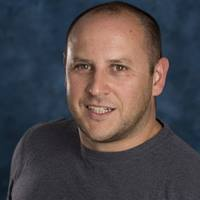
\includegraphics[width=8.5cm]{error.jpg}

    \textbf{Figure 7 Error page}
    \vspace{2mm}

    \begin{lstlisting}[caption = How error pages are handled]
    @app.errorhandler(404)
    def page_not_found(e):
        return render_template('404error.html'), 404
    \end{lstlisting}

    For the login functionality I used an object called session which allows me to store information specific to a user from one request to another[7]. I included a secret key to make sure that even though the user could look at the contents of my cookie, they can't modify it unless they know the secret key used for signing. To create the secret key I used python's \textit{urandom(size)} which returns a string of size random bytes suitable for cryptographic use[8].

    \begin{lstlisting}[caption = How secret key is created]
    app = Flask(__name__)
    app.secret_key = os.urandom(12)
    \end{lstlisting}

    Something that makes my web-app efficient is that there are no repeated loops in my code. If something is repeated twice, a function could make it only appear once. For example, the way I retrieve information from the JSON files is through a function called \textit{findFood(search)} through which I pass the object to find. This was useful since those objects can be found from anywhere in the web, and if the object was not found, an appropriate error handler initiated. Another function called \textit{generateID(filename)} takes in a JSON file, and generates the next id number making sure none of them are repeated and overlapped. This way I was able to add objects to the files without any crashes.

    Another useful functionality is that users are able to download a pdf file containing information about healthy eating. The file is saved in the static folder and is accessed when the user either clicks a button or writes the specific URL:

    \begin{lstlisting}[caption = Downloading files]
    @app.route('/mealplan/pyramid/', methods=['GET'])
    def pyramid():
    if request.method == 'GET':
        return send_from_directory(directory='static/files/', filename='pyramid.pdf')
    \end{lstlisting}

    All websites should have authority (who developed the site), purpose, coverage (if topics are explored in depth), be current (how up-to-date the information is), objectivity (if the information biased) and accuracy (if the author is related to a known, respectable institution, no grammar or spelling mistakes...).

    This web-app has authority and shows the author (me) in the footer on the index page. It doesn't show it in the rest of the pages because it does not follow the design pattern that I first designed. There is no contact information such as email or phone number since there is a Contact page where the user can directly contact the admin without having to use a different email page.

    The purpose of the web is to \textbf{inform} about the importance of Realfooding, eating real food instead of ultra-processed aliments. The information isn't geared to a specific audience. It contains valuable information that adults and teenagers will find useful, while also making use of diagrams that make the web more entertaining for kids. It is also easy to read, therefore kids will not find it boring and exhausting and they might learn something useful.

    The information provided is of a wide range and comprises many useful links and possible pathways. None of the links go to outside sites rather than its own since all the information it requires is saved in the JSON files and more can be added when needed very easily.

    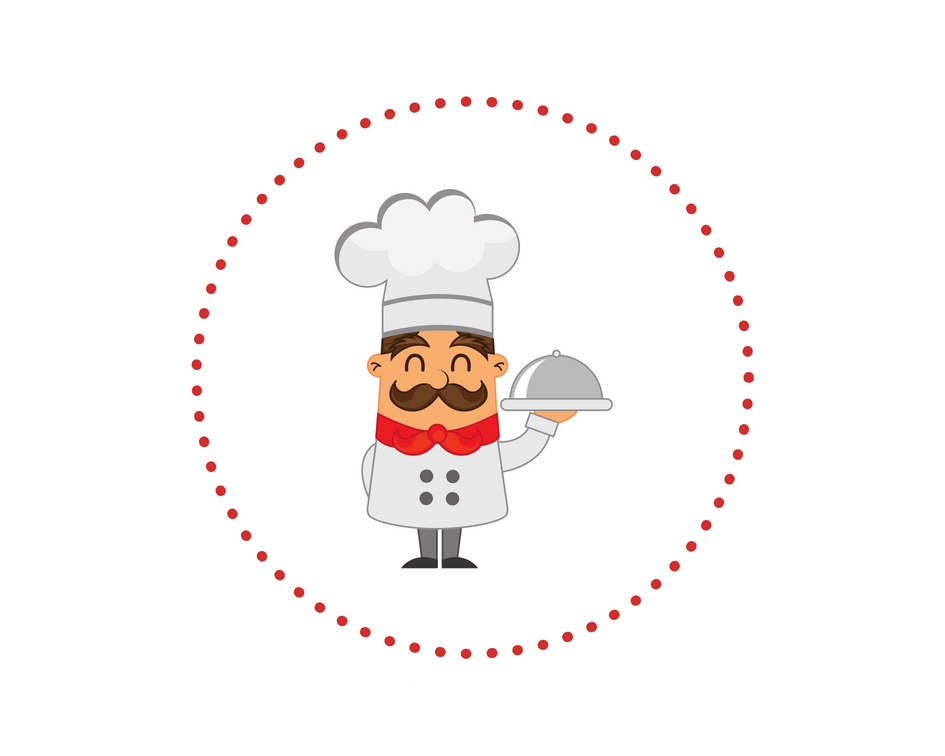
\includegraphics[width=8.5cm]{images/recipes.jpg}

    \textbf{Figure 8 Recipes page}
    \vspace{2mm}

    The 'Add recipe' button will only appear if the admin is logged in. The users won't be able to view it. This also makes the web current, since it will always be up to date if the admin keeps renovating the information.


    \section{Personal Evaluation}

    Thanks to this coursework, I have learned about how powerful Python is when it comes to web development and more about JSON files, which I already knew about but never really understood them as well as now. It also broadened my knowledge of CSS and Bootstrap, as I first started this coursework using Bootstrap, and then I felt it would be more unique and personalised if I designed my own CSS.

    It wasn't hard to start since the Workbook provided for the course contains most of the basic things we needed to create the coursework. However, to add more complicated features I downloaded various flask examples which I read and analysed so I could then implement in my own web.

    After doing this coursework I feel like I learned a lot, but there is still so much more left for me to learn and I can't wait to start another project soon.

    Overall, I am very happy with my web. It has many functionalities and in my opinion, the layout is very aesthetically pleasing.

    \section{References}

    [1]

    \url{https://cdn1.sph.harvard.edu/wp-content/uploads/sites/30/2012/10/healthy-eating-pyramid-huds-handouts.pdf}

    [2] Designing Web Applications

    \url{http://nathanbarry.com/webapps/}

    [3]
    \url{https://www.canva.com/}

    [4]

    \url{https://lh3.googleusercontent.com/b1_u9EJmEcMMx3NFdzv122hs4CBnxrDFlw0Z6Xny0mgRhqCCasoLTFKb-FH7-N3ttxnE=s127}

    [5]

    \url{https://tsquaredmarketing.com/website-enhancement/}

    [6]

    \url{https://lrweb.beds.ac.uk/applied-soc-studies/Webresources/evaluate-a-webpage}

    \url{https://cdn.dal.ca/content/dam/dalhousie/pdf/library/CoreSkills/6_Criteria_for_Websites.pdf}

    [7]

    \url{http://flask.pocoo.org/docs/1.0/quickstart/}

    [8]

    \url{https://docs.python.org/3/library/os.html}

    Website information came from:

    \url{https://en.wikipedia.org/wiki/Fruit#Nutritional_value}

    \url{https://www.healthline.com/nutrition/how-much-fruit-per-day}

    \url{https://iplaybaby.com/whole-baby-resource/info/types-of-fruits/}

    \url{https://www.vegetables.co.nz/vegetables-a-z/}

    \url{https://www.quora.com/Why-do-we-need-to-eat-vegetables}

    \url{http://www.carballeira.com/en/white-fish-or-blue-fish/}

    \url{https://www.safefood.eu/Healthy-Eating/What-is-a-balanced-diet/The-Food-Pyrami/Breads,-cereals-and-potatoes.aspx}

    \url{https://mindovermunch.com/2018/05/03/are-processed-foods-bad/}

    \url{https://www.sproutright.com/blog/index.php/5-reasons-you-need-snacks/}

    \section{Appendices}

    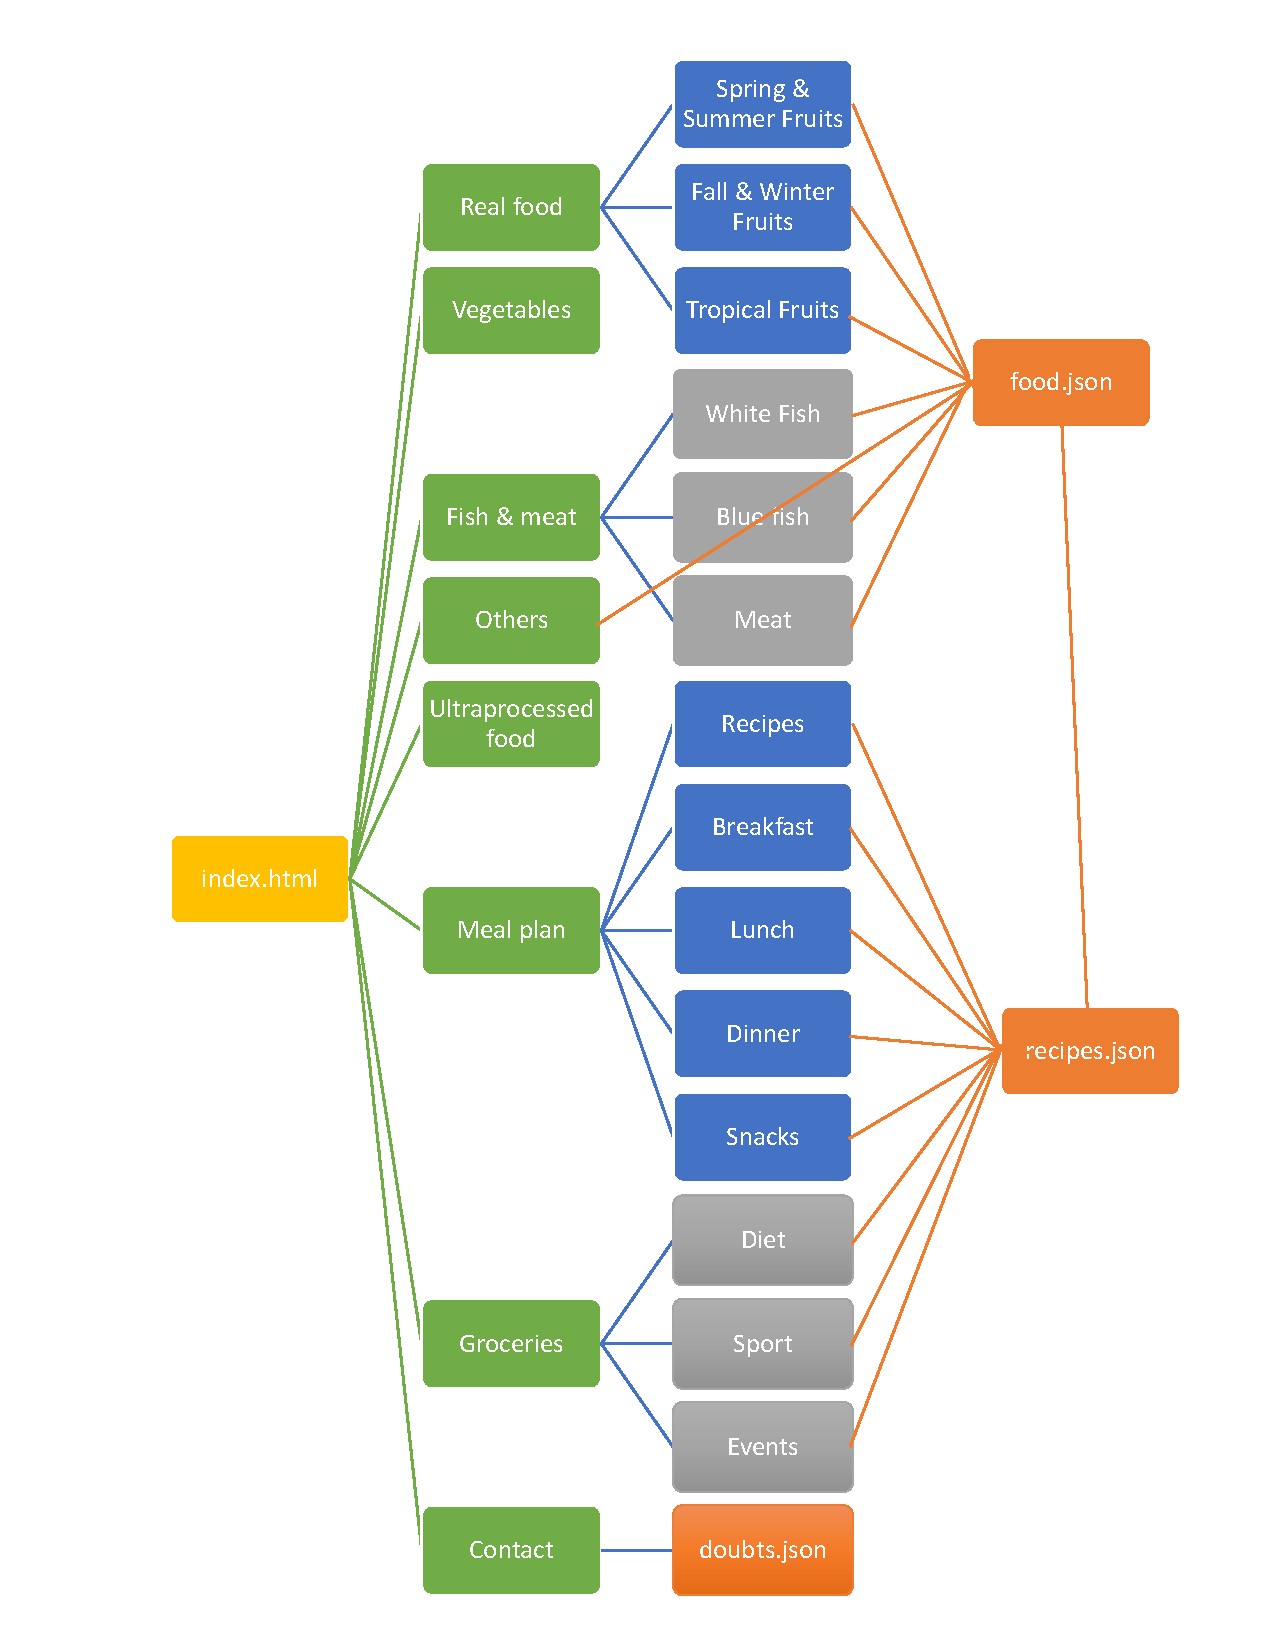
\includegraphics[width=8cm]{images/hierarchy.pdf}

    \textbf{Appendix 1 Navigation diagram}
    \vspace{2mm}

\end{document}
